

\section{利用者の管理とアクセス制御システムの整備}\label{4.2}
独立した運用を行うためには利用者の管理とアクセス制御システムの整備が必要である.
既存の滞在ウォッチは単独コミュニティでのみの運用を前提としており開発者と管理者が同一であった.Web上からユーザの登録をするシステムが存在せず開発者がデータベースに対して直接変更を行うSQLを発行していた.
これは単一コミュニティでの運用であったため成り立っていたが,複数コミュニティ間で運用を行う場合,コミュニティの数が増えるに連れてシステム開発者の利用者管理の負担が大きくなり運用するのは難しくなる.
また在室者情報はプライバシに関わるため,部外者がWebページにアクセスしても在室者情報を閲覧できないようにする必要があるにも関わらず,誰でも閲覧可能な状態であった.
これらを解決するには利用者のアクセス制御システムの整備とコミュニティごとの管理者を作り,各コミュニティで独立した運用を行う必要がある.
各コミュニティごとに管理者が存在すればコミュニティの利用者の管理を開発者が全て行う必要がないため負担が軽減される.


そこでFirebase AuthenticationのGoogleプロバイダーによるOAuth認証を実装した.
OAuth (Open Authorization)は,ユーザーがサービスプロバイダー(例えばGoogle,FaceBookなど)に対して,別のサービスにアクセスするための権限を与えるためのオープンスタンダードの認証プロトコルである.
OAuth以外の認証方式としてBasic認証などがある.Basic認証はユーザ名とパスワードをベーシック認証ヘッダーに埋め込んで送信する方式である.この方式はセキュリティ上の問題が存在する.パスワードが暗号化されていないため,パスワードが盗まれる危険がある.また,Basic認証はバックエンド側でユーザ名とパスワードを保存する必要があり,管理を行うにはパスワードのハッシュ化など適切な処理を施す必要がある.
それと比較してOAuth認証では,ユーザのアカウント情報を第三者にアプリケーションに渡さずにアクセス権を付与できるため,セキュリティ上の利点がある.
OAuth認証では,アクセス権を持つアプリケーションにのみ有効で,期限切れになると,使用できなくなる.これにより,アクセス権を付与したアプリケーションが不正にアクセスするのを防止できる.
これらの理由により,OAtuh認証を採用した.
OAuthプロバイダーにはApple,FaceBookなど複数の選択肢がある中でGoogleを採用した.Googleアカウントは世界中で広く利用されており,多くの人がアカウントを持っており,多数の利用者に対応可能である.

Googleアカウントを用いたOAuth認証は,Googleアカウントを使って,サービスプロバイダー(Google)に対して,利用者が滞在ウォッチシステムにアクセスするための権限を与える.利用者はGoogleアカウントにログインし,Googleが提供するOAuth認証プロセスを通じて,滞在ウォッチシステムにアクセスできる.
OAuth認証により,利用者は自分のGoogleアカウントの情報(パスワードなど)を滞在ウォッチシステムに入力をせずに,安全にアクセスできる.
しかしGoogleアカウントによるOAuth認証だけでは意図しない外部のユーザのアクセスを防ぐことはできない.なぜならGoogleアカウントを持っているユーザなら誰でも認証を行えるためである.
そこでGoogleアカウントによるOAuth認証に加えて滞在ウォッチサーバ側で独自のユーザ認証を行った.具体的には滞在ウォッチ管理者が登録したユーザのみを認証するというものである.滞在ウォッチサーバのデータベースにはGoogleのアカウントのユーザ名であるメールアドレスが保存してある.この保存されたメールアドレスは滞在ウォッチの管理者が登録したものであるため,メールアドレスが存在する場合は管理者の許可のある正規のユーザと判別できる.



管理者のユーザ登録フロー図を図\ref{fig:registerUser}に示し具体的に説明する.
まず初めに利用者は管理者に対してGoogleアカウントを報告する.
報告後管理者がWebの管理者ページのユーザ登録画面からGoogleアカウントを登録する.
ユーザには2種類のパターンが想定される.

\begin{figure}[h]
  \centering  % 図を真ん中に配置
  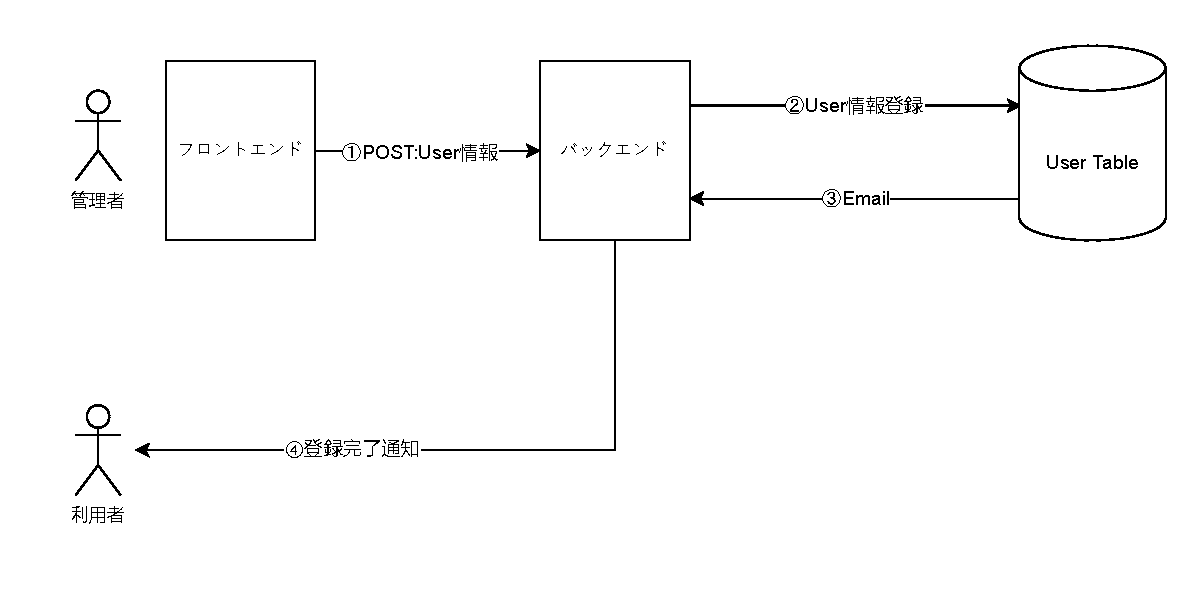
\includegraphics[clip,scale = 0.7]{image/regsiterUser.pdf}
  \caption{認証システム:管理者側のユーザ登録フロー図}    \label{fig:registerUser}
\end{figure}



% \begin{figure}[tbh]
%   \centering
%   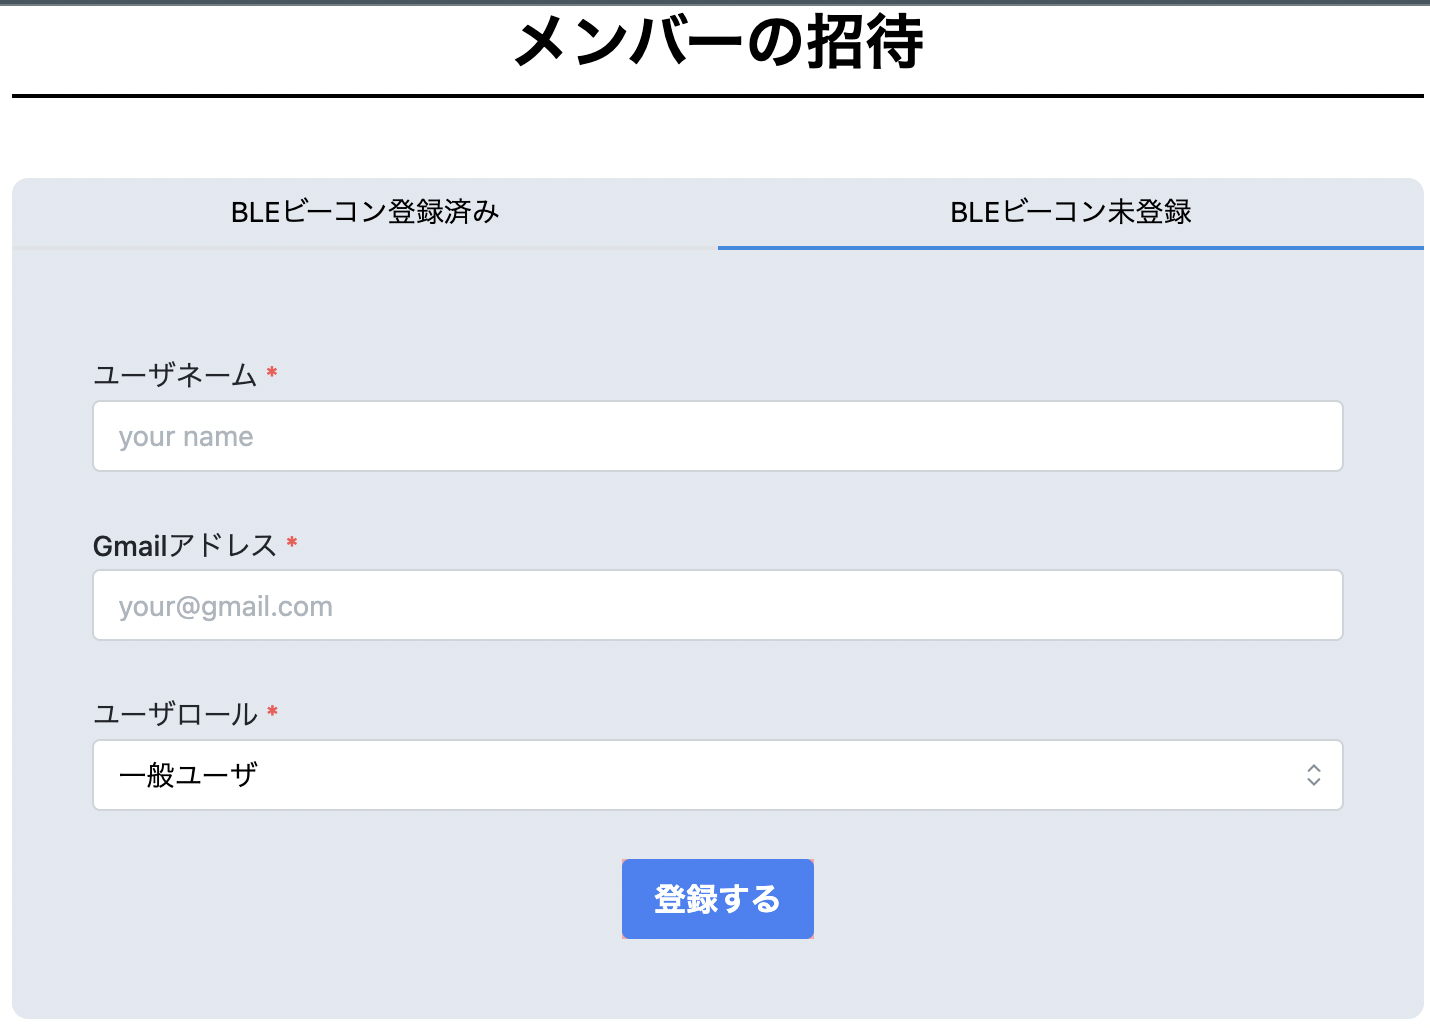
\includegraphics[width=16cm]{image/registerNotBLE.png}
%   \caption{BLEビーコン未登録} \label{fig:registerNotBLE}
%   \label{multipleBPM}
% \end{figure}
まず1つ目はBLEビーコンが既に登録済みのユーザ場合の登録である.
図\ref{fig:registerBLE}にその登録画面を示す.
この登録画面は以前から滞在ウォッチユーザとして登録がされておりビーコンに関する情報とユーザ情報が既に存在するが,Googleアカウントの情報とユーザロールがないユーザを想定している.
ユーザネームはデータベースに存在しているためバックエンドからデータを取得できる.
この登録画面は,以前から「滞在ウォッチユーザ」として登録されているユーザ向けで,ビーコンに関する情報やユーザネームの情報は既に存在しており,Google アカウントの情報やユーザロールのみがないユーザを対象としている.
取得した利用者のユーザネームデータを管理者が選択できるようにセレクトボックスを配置した.
ユーザロールのところでユーザの権限レベルの指定ができる.
一般ユーザと管理者ユーザの2つがあり,一般ユーザは滞在ウォッチの在室者情報の閲覧などを行え,管理者ユーザは一般ユーザの権限に加えてユーザの登録を行える.
管理者が登録ボタンを押すと,POSTリクエストがサーバ側に送信される.
登録されると管理者が選択したデータベースに存在するユーザにメールアドレスが紐づき,サーバ側は対象のメールアドレスに対して登録完了のメールを送信する.メールアドレスに対して通知を行うのはユーザがいつ登録が完了したのか把握できるようにするためである.
2つ目に想定されるのがビーコンが登録されていない新規ユーザである.登録画面を図\ref{fig:registerNotBLE}に示す.ユーザは\ref{4.3}章で説明するスマホビーコンを使用する新規ユーザである.新規ユーザにはユーザネームがないため管理者はユーザネームを入力する必要がある.その他は先に述べた登録画面と同じであり,登録ボタンを押しサーバに対してリクエストを送信する.
先に述べたものとの違いはサーバ側は新規のUUIDの生成を行うところである.
スマホビーコンの初期セットアップ時にUUIDの設定を行う,
その際ユーザのGoogleアカウントに対応したUUIDをセットアップできる.


\begin{figure}[tbh]
  \centering
  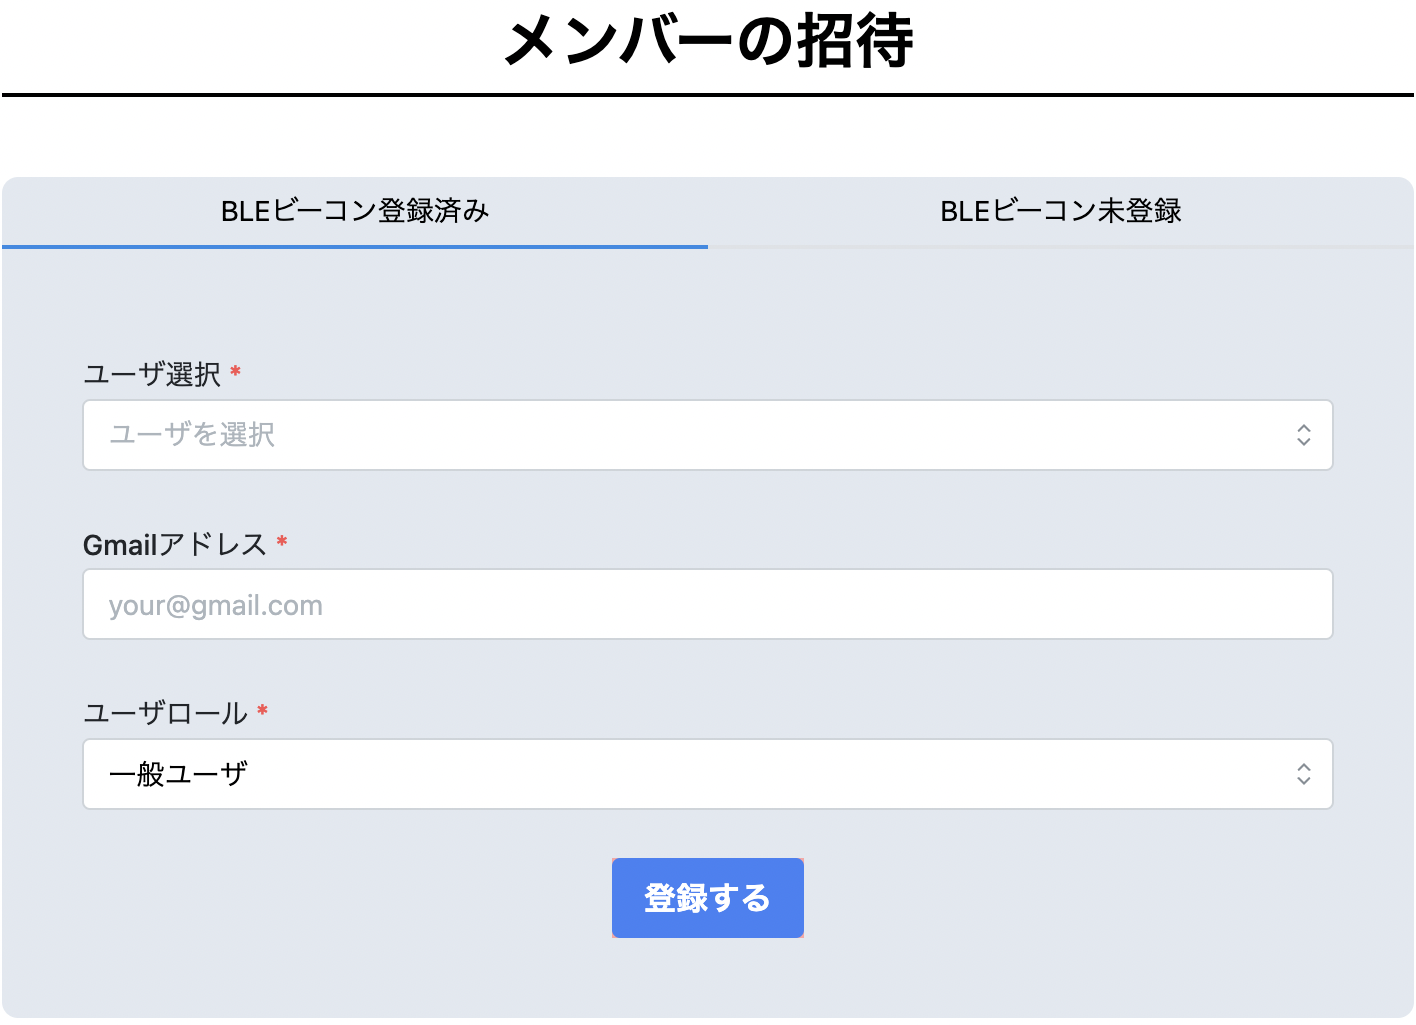
\includegraphics[width=16cm]{image/registerBLE.png}
  \caption{BLEビーコン登録済みの登録画面} \label{fig:registerBLE}

\end{figure}

\begin{figure}[tbh]
  \centering
  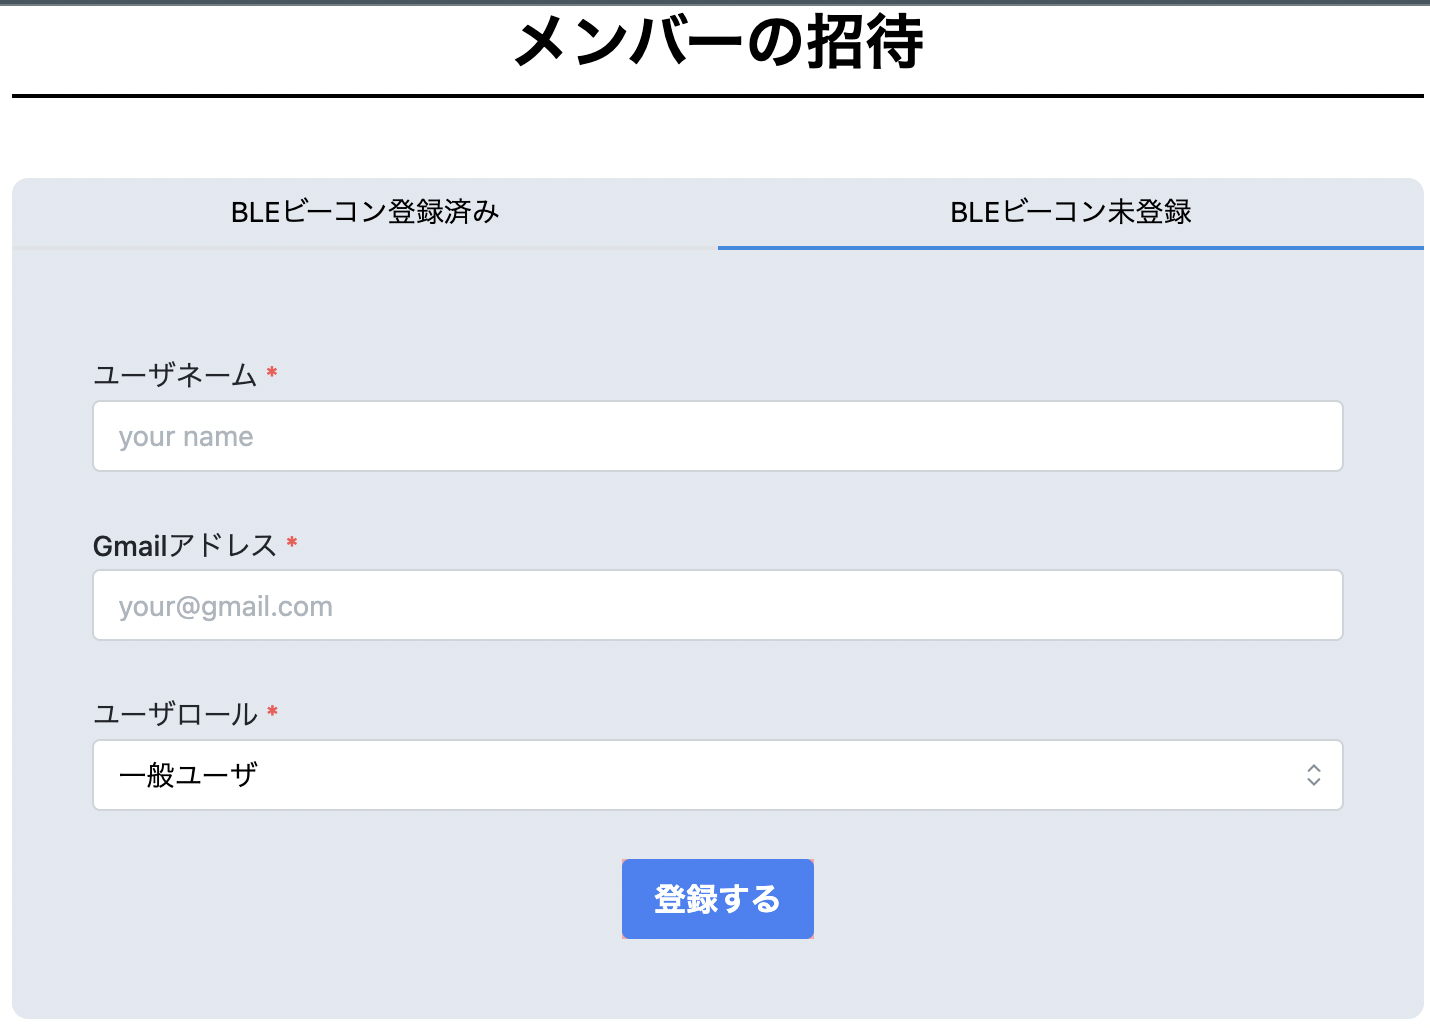
\includegraphics[width=16cm]{image/registerNotBLE.png}
  \caption{BLEビーコン未登録の登録画面} \label{fig:registerNotBLE}

\end{figure}


\newpage


次にユーザ側の認証のフローを\ref{fig:userLogin}説明する.
Fireabase Authで認証が成功するとJWT(JSON Web Token)トークンが発行される.Firebase AuthのJWTトークン はFirebase Authが認証済みのユーザーを確認するために使用するトークンである.
JWTトークンは,JSON形式の文字列では発行者,トークンの有効期限,トークンの使用目的,サブジェクトが含まれておりユーザを一意に識別可能である.
JWTトークンは,フロントエンドから滞在ウォッチのバックエンドに送信される.
滞在ウォッチのバックエンドはFirebase AuthのAPIを使用して,JWTトークンの検証を行い,トークンが有効であるか確認する.有効なJWTトークンであった場合,アプリケーションのバックエンドは,そのトークンに含まれる情報を使用して,Firabase Authが認証済みであることを確認する.認証済みであった場合は次にメールアドレス情報を確認する.
データベースにメールアドレスが存在する場合フロントエンドに対してアクセスの許可を行うResponse Code 200を返す.
このプロセスによって不正なユーザの在室者の閲覧を防いでいる.よって適切な範囲での在室者情報の共有が可能である.



\newpage

\begin{figure}[h]
  \centering  % 図を真ん中に配置
  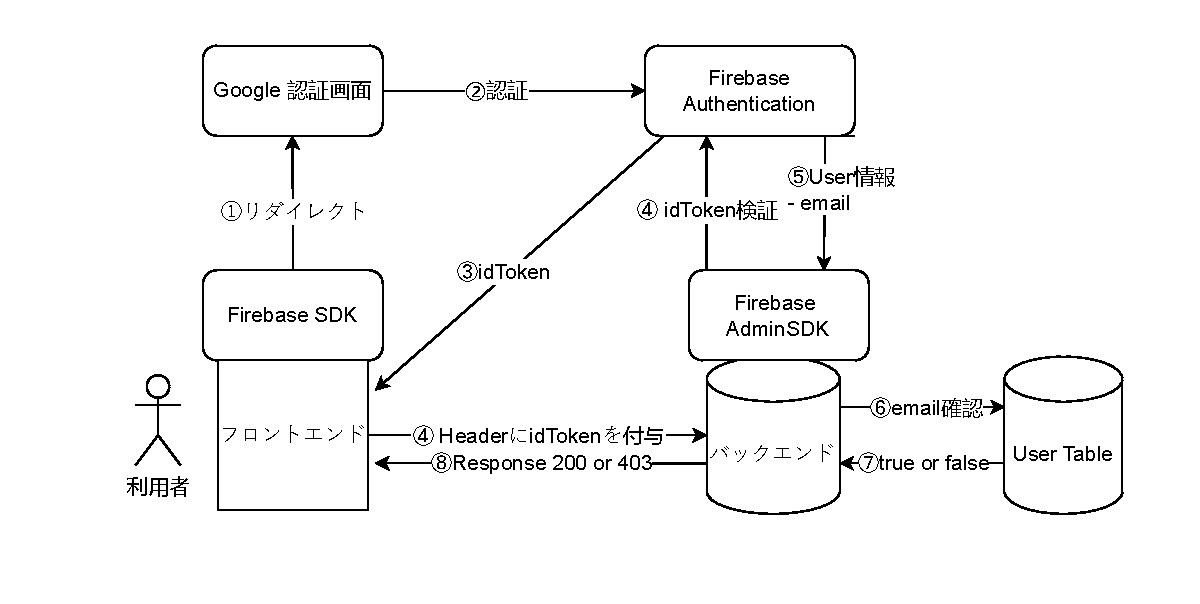
\includegraphics[clip,scale = 0.8]{image/userLogin.pdf}
  \caption{認証システム: ユーザ側のフロー図}    \label{fig:userLogin}
\end{figure}


